\documentclass[12pt]{article}

\usepackage[default]{lato}
\usepackage[T1]{fontenc}
\usepackage{graphicx}
\usepackage{blindtext}
\usepackage{listings}
\def\arraystretch{1.5}%

\usepackage{subfig}
\usepackage{tikz}
\usetikzlibrary{positioning, matrix, arrows.meta,calc}

\usepackage[font=small,labelfont=bf, justification=justified, format=plain]{caption}
\tolerance=1
\emergencystretch=\maxdimen
\hyphenpenalty=10000
\hbadness=10000


\usepackage{hyperref}
\hypersetup{
	colorlinks,
	citecolor=black,
	filecolor=black,
	linkcolor=black,
	urlcolor=black
}

\renewcommand{\contentsname}{Spis treści}
\renewcommand{\figurename}{Ilustracja nr.}
\renewcommand{\lstlistingname}{Skrypt nr.}
\lstset{ 
	basicstyle=\footnotesize, frame=tb,
	xleftmargin=.2\textwidth, xrightmargin=.2\textwidth
}
\usepackage[margin=2cm]{geometry}

\lstdefinestyle{tt}{basicstyle=\small\ttfamily,keywordstyle=\bfseries,language=[LaTeX]{TeX}}
\lstdefinestyle{rm}{basicstyle=\ttfamily,keywordstyle=\slshape,language=[LaTeX]{TeX}}

\title{}
\author{}
\date{}

\begin{document}
	\begin{titlepage}
		\centering
		\vspace{1cm}
		{\huge\bfseries Systemy cyfrowe i komputerowe\par}
		\vspace{0.5cm}
		{\huge\bfseries Dokumentacja projektu ``exe\_unit\_w1''\par}
		\vspace{2cm}
		{\Large\itshape Karol Ambroziński\par}
		\vspace{0cm}
		{\Large\itshape Nr. albumu: 318488\par}
		\vfill
	\end{titlepage}

	\tableofcontents
	
	\newpage
	
	\section{Wejścia, wyjścia, parametry i zakresy ich wartości}
	
	\subsection{Parametry}
\begin{itemize}
	\item \emph{\textbf{m}} - określa wielkość w bitach główne wejścia i wyjścia danych,
	\item \emph{\textbf{n}} - określa ilość operacji.
\end{itemize}

\subsection{Wejścia}

\begin{itemize}
	\item \emph{\textbf{i\_oper}} - n-bitowe wejście określające wykonywaną operację,
	\item \emph{\textbf{i\_argA}} - m-bitowe wejście; kodowanie ZNAK-MODUŁ,
	\item \emph{\textbf{i\_argB}} - m-bitowe wejście; kodowanie ZNAK-MODUŁ,
	\item \emph{\textbf{i\_clk}} - 1 bitowe wejście zegarowe,
	\item \emph{\textbf{i\_rsn}} - 1 bitowe wejście resetu synchronicznego.
\end{itemize}

\subsection{Wyjścia}
\begin{itemize}
	\item \emph{\textbf{o\_status}} - m-bitowe wyjście,
	\item \emph{\textbf{o\_result}} - 4 bitowe wyjście; kodowanie ZNAK-MODUŁ lub U2.
\end{itemize}


	
	\section{Realizowane funkcje i ich argumenty}

	Układ realizuje 4 operacje (4 podmoduły):

\subsection{Podmoduł \emph{mod1}:}
Odejmowanie argumentów (A - B); jeśli operacja nie może zostać wykonana, jednostka zgłasza błąd, a wyjście jest niezdefiniowane.

\subsubsection*{Wejścia}
\begin{itemize}
	\item i\_argA - m-bitowe wejście,
	\item i\_argB - m-bitowe wejście,
\end{itemize}
\subsubsection*{Wyjścia}
\begin{itemize}
	\item o\_result - m-bitowe wyjście,
	\item o\_status - 4 bitowe wyjście.
\end{itemize}

\subsection{Podmoduł \emph{mod2}:}
Porównanie argumentów (A < B); jeśli warunek jest spełniony to wynikiem jest liczba 1, w przeciwnym wypadku wynikiem jest 0,

\subsubsection*{Wejścia}
\begin{itemize}
	\item i\_argA - m-bitowe wejście,
	\item i\_argB - m-bitowe wejście,
\end{itemize}
\subsubsection*{Wyjścia}
\begin{itemize}
	\item o\_result - m-bitowe wyjście,
	\item o\_status - 4 bitowe wyjście.
\end{itemize}

\subsection{Podmoduł \emph{mod3}:}
Ustawienie bitu w argumencie A na wartość 0; numer bitu jest określony w argumencie B; zgłoszenie błędu jeśli wartość B jest ujemna lub przekrasza liczbę bitów argumentu A,

\subsubsection*{Wejścia}
\begin{itemize}
	\item i\_argA - m-bitowe wejście,
	\item i\_argB - m-bitowe wejście,
\end{itemize}
\subsubsection*{Wyjścia}
\begin{itemize}
	\item o\_result - m-bitowe wyjście,
	\item o\_status - 4 bitowe wyjście.
\end{itemize}

\subsection{Podmoduł \emph{mod4}:}
Konwersja argumentu A z kodu ZNAK-MODUŁ na U2; jeśli konwersja nie może zostać wykonana - zgłaszany jest błąd a wynik jest nieokreślony.

\subsubsection*{Wejścia}
\begin{itemize}
	\item i\_argA - m-bitowe wejście,
\end{itemize}
\subsubsection*{Wyjścia}
\begin{itemize}
	\item o\_result - m-bitowe wyjście,
	\item o\_status - 4 bitowe wyjście.
\end{itemize}
	
	\section{Schemat blokowy struktury jednostki}
	
		\begin{figure}[htb]
	\centering
	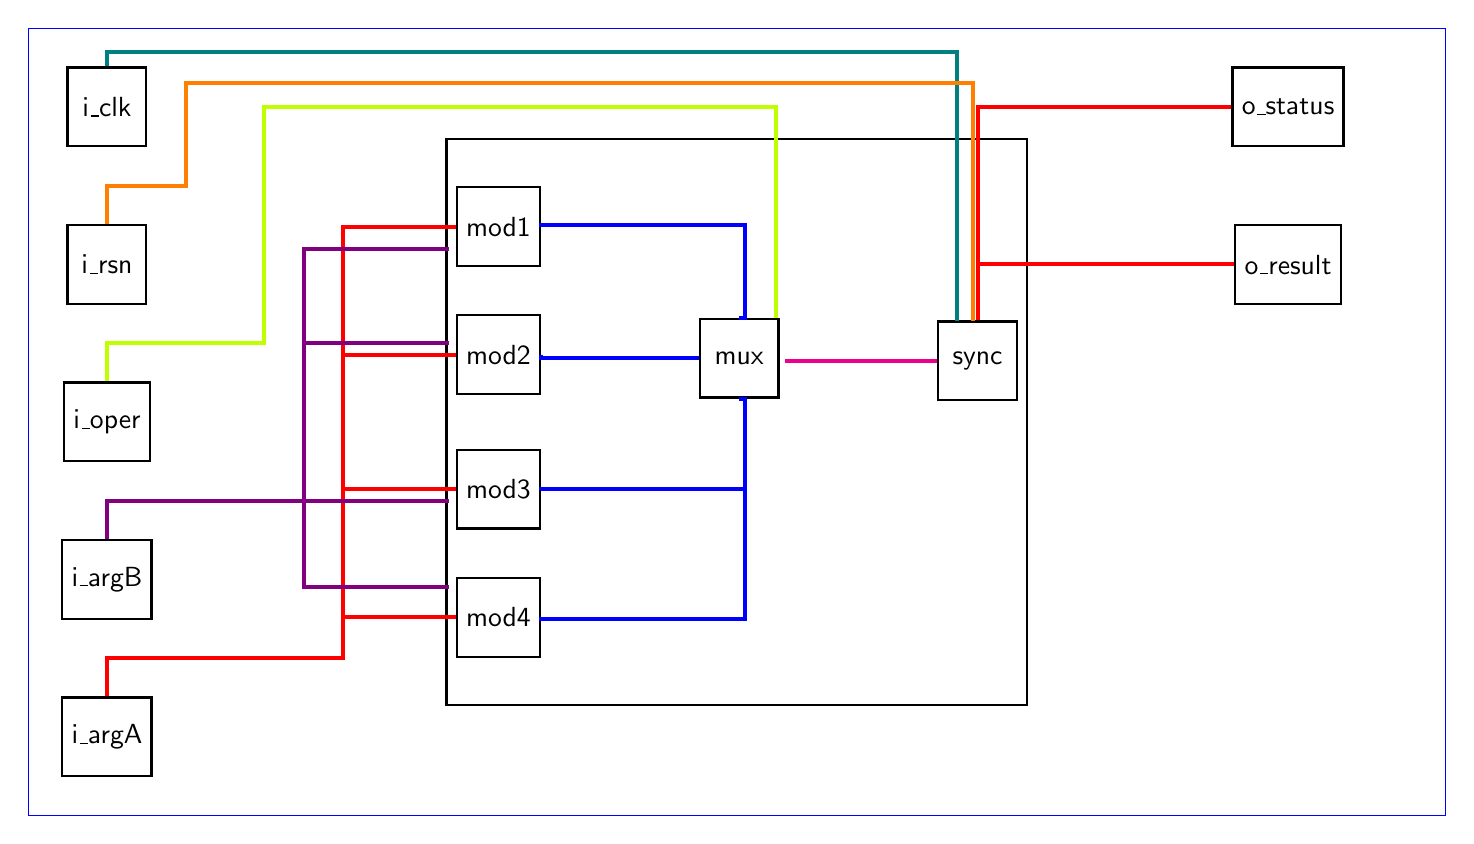
\begin{tikzpicture}[
		myline/.style={draw=black!40!black, thick},
		box/.style={myline, minimum height=1cm, minimum width=1cm, font=\sffamily, inner sep=.3333em}, >=Stealth]
		
		\draw [blue] (-11,-1) rectangle (7,9);
		
		\matrix (ALU) [matrix of nodes, inner ysep=6mm, nodes=box, myline, column sep=20mm, row sep = 6mm] at (-2,4)
		{|(mod1)|mod1 \\ |(mod2)|mod2 & |(mux)|mux & |(sync)|sync \\ |(mod3)|mod3 \\ |(mod4)|mod4 \\};
		
		
		
		\node[box] at (-10,0)  (argA) {i\_argA};
		\node[box] at (-10, 2) (argB) {i\_argB};
		\node[box] at (-10,4)  (oper) {i\_oper};
		\node[box] at (-10,6)  (rsn) {i\_rsn};
		\node[box] at (-10,8)  (clk) {i\_clk};
		
		\node[box] at (5,6)  (result) {o\_result};
		\node[box] at (5,8)  (status) {o\_status};
		
		\draw[-, red, line width=0.5mm]  (argA)|-(-10, 1)|-(-7, 1)|-(-7, 6)|-(mod1);
		\draw[-, red, line width=0.5mm]  (argA)|-(-10, 1)|-(-7, 1)|-(-7, 4)|-(mod2);;
		\draw[-, red, line width=0.5mm]  (argA)|-(-10, 1)|-(-7, 1)|-(-7, 2)|-(mod3);
		\draw[-, red, line width=0.5mm]  (argA)|-(-10, 1)|-(-7, 1)|-(-7, 1)|-(mod4);
		\draw[-, red, line width=0.5mm]  (sync)|-(result);	
		\draw[-, red, line width=0.5mm]  (sync)|-(status);
		
		\draw[-, red, line width=0.5mm]  (argA)|-(-10, 1)|-(-7, 1)|-(-7, 6)|-(mod1);
		\draw[-, red, line width=0.5mm]  (argA)|-(-10, 1)|-(-7, 1)|-(-7, 4)|-(mod2);
		\draw[-, red, line width=0.5mm]  (argA)|-(-10, 1)|-(-7, 1)|-(-7, 2)|-(mod3);
		\draw[-, red, line width=0.5mm]  (argA)|-(-10, 1)|-(-7, 1)|-(-7, 1)|-(mod4);
		
		%\draw[-, blue, line width=0.5mm]  (argB)|-(-10, 3)|-(-7.5, 3)|-(-7.5, 3)|-(-7.5, 1.8)|-(-5.64, 1.8);
		%\draw[-, violet, line width=0.5mm]  (argB)|-(-10, 3)|-(-7.5, 3)
		\draw[-, violet, line width=0.5mm]  (argB)|-(-10, 3)|-(-7.5, 3)|-(-7.5, 1.9)|-(-5.65, 1.9);
		\draw[-, violet, line width=0.5mm]  (argB)|-(-10, 3)|-(-7.5, 3)|-(-5.65, 3);
		\draw[-, violet, line width=0.5mm]  (argB)|-(-10, 3)|-(-7.5, 3)|-(-7.5, 5)|-(-5.65, 5);
		\draw[-, violet, line width=0.5mm]  (argB)|-(-10, 3)|-(-7.5, 3)|-(-7.5, 6.2)|-(-5.65, 6.2);;
		
		\draw[-, lime, line width=0.5mm]  (oper)|-(-8, 5)|-(-8, 8)|-(-1.5, 8)|-(-1.5, 5.32);
		
		\draw[-, teal, line width=0.5mm]  (clk)|-(-8, 8.7)|-(0.8, 8.7)|-(0.8, 5.28);
		
		\draw[-, orange, line width=0.5mm]  (rsn)|-(-9, 7)|-(-9, 8.3)|-(1, 8.3)|-(1, 5.28);
		
		\draw[-, magenta, line width=0.5mm]  (-1.37,4.75)|-(sync.west);
		\draw[-, blue, line width=0.5mm]  (mod2.east)|-(mux);
		\draw[-, blue, line width=0.5mm]  (mod3.east)|-(-1.9, 3.15)|-(mux.south);
		\draw[-, blue, line width=0.5mm]  (mod4.east)|-(-1.9, 1.5)|-(mux.south);
		\draw[-, blue, line width=0.5mm]  (mod1.east)|-(-1.9, 6.5)|-(mux.north);
	\end{tikzpicture}
	\caption{Schemat blokowy \textbf{\emph{exe\_unit\_w1}}}
\end{figure}
	
	\section{Sygnały zaimplementowanych flag i ich wartości}
	
	Zaimplementowane flagi o\_status:

\begin{itemize}
	\item ERROR - operacja nie została wykonana - o\_result jest nieokreślone; pierwszy bit o\_status od prawej jest równy 1,
	\item NEG - wynik jest liczbą ujemną; drugi bit o\_status od prawej jest równy 1,
	\item EVEN - w wyniku jest parzysta liczba jedynek; trzeci bit o\_status od prawej jest równy 1,
	\item ONES - wszystkie bity o\_result ustawione; ostatni bit o\_status od prawej jest równy 1,
\end{itemize}

\noindent
Jeśli wynik jest nieokreslony (flaga ERROR) to pozostałe bity nie są ustawiane; warunki pozostałych flag nie są sprawdzane.

	\newpage

	\section{Przykład użycia modułu}
	\subsection{Przykład nr. 1}

\noindent
Na ilustracji nr. 2 przedstawiono wykonanie dwóch operacji: odejmowanie liczb A i B oraz zmianę bitu w argumencie A oznaczonego indeksem B (moduły: \textbf{\emph{mod1}} i \textbf{\emph{mod3}}). Przy pierwszej operacji na początku wynik jest niezdefiniowany i flaga błędu ustawiona na 1; przepełnienie wartości. W kolejnej operacji w argumencie B został zmieniony bit na indeksie B: B równe jest \(3_{10}\), więc bit nr. \(3_{10}\) (liczony od \(0_{10}\)) w A został zmieniony na \(0_2\). Przy operacji ustawiania bitu poprzez B widać ustawienie flagi \(0100_2\) która oznacza że wynik posiada parzystą liczbę jedynek (co też jest widoczne na wyjściu \textbf{\emph{o\_result}}).

\begin{figure}[h!]
	\centering
	\includegraphics[width=1\linewidth]{img1}
	\caption{Widok wykonania testbenchu RTL i oryginalnych plikow w GTKWave}
	\label{fig:img1}
\end{figure}

\subsection{Przykład nr. 2}

\noindent
Na ilustracji nr. 3 wykonywane są dwie operacje: porównanie liczb A i B oraz konwersja liczby w kodowaniu ZNAK-MODUŁ na U2 (moduły: \textbf{\emph{mod2}} i \textbf{\emph{mod4}}). Na początku liczba A jest większa od liczby B (liczba A jest dodatnia, a liczba B jest ujemna) więc na wyjściu jest \(0_{ZM}\). Przy następnych wartościach A i B (A mniejsze od B) wyjście równe jest \(1_{10}\). Następnie zmieniana jest operacja (ZM na U2) gdzie wejście A równe jest \(1011_{ZM}\) które pózniej konwertowane jest na \(1101_{U2}\). Po tej konwersji na wejście podane jest ujemne zero (\(1000_{ZM}\)) które dla \textbf{\emph{mod4}} jest błędem, więc flaga \textbf{\emph{o\_status}} ustawiana jest na \(0001_{2}\), a wyjście jest niezdefiniowane.

\begin{figure}[h!]
	\centering
	\includegraphics[width=1\linewidth]{img2}
	\caption{Widok wykonania testbenchu RTL i oryginalnych plikow w GTKWave}
	\label{fig:img1}
\end{figure}

\newpage

\subsection{Przykład nr. 3}

Na ilustracji nr. 4 widać wykonywanie operacji odejmowania liczb A - B oraz zamianę liczby A z kodowanie ZNAK-MODUŁ na U2 (moduły: \textbf{\emph{mod1}} i \textbf{\emph{mod4}}). Na początku A ma wartość \(1111_{ZM}\) a B \(0000_{ZM}\), więc ich różnica równa jest początkowemu A; widać tutaj ustawienie wszystkich flag \textbf{\emph{o\_status}}, oprócz bitu \textbf{\emph{ERROR}}. Następnie mzieniane są wartości A i B, których różnica powoduje przepełnienie, więc błąd (wyjście - niezdefiniowane, a flaga \textbf{\emph{ERROR}} ustawiona na \(1_2\)). W kolejnym takcie zegara, zmianie ulega wejście A oraz operacja na zamianę kodowanie z ZNAK-MODUŁ na U2: wartość \(1011_{ZM}\) zamieniana jest na \(1101_{U2}\). Pózniej zmieniana jest wartość A na ujemne zero (\(1000_{ZM}\)); błąd - wyjście niezdefiniowane.

\begin{figure}[h!]
	\centering
	\includegraphics[width=1\linewidth]{img3}
	\caption{Widok wykonania testbenchu RTL i oryginalnych plikow w GTKWave}
	\label{fig:img1}
\end{figure}

	\section{Lista plików}
	\begin{itemize}
	\item exe\_unit\_w1.sv - plik zawierający ALU,
	\item otherModules.sv - plik zawierający wszystkie podmoduły ALU,
	\item exe\_unit\_w1\_rtl.sv - plik ALU po syntezie,
	\item synth.log - raport Yosysa po syntezie.
\end{itemize}
	\newpage
	\section{Raport z syntezy logicznej}
	\begin{table}[!htb]
	\begin{minipage}{0.55\linewidth}
		\centering
		\begin{tabular}{lllll}
			\cline{1-2}
			\multicolumn{2}{|c|}{\textbf{Podmoduł \emph{mod1}}} &  &  &  \\ \cline{1-2}
			\multicolumn{1}{|l|}{Number of wires:} & \multicolumn{1}{c|}{88} &  &  &  \\ \cline{1-2}
			\multicolumn{1}{|l|}{Number of wire bits:} & \multicolumn{1}{c|}{115} &  &  &  \\ \cline{1-2}
			\multicolumn{1}{|l|}{Number of public wires:} & \multicolumn{1}{c|}{12} &  &  &  \\ \cline{1-2}
			\multicolumn{1}{|l|}{Number of public wire bits:} & \multicolumn{1}{c|}{39} &  &  &  \\ \cline{1-2}
			\multicolumn{1}{|l|}{Number of memories:} & \multicolumn{1}{c|}{0} &  &  &  \\ \cline{1-2}
			\multicolumn{1}{|l|}{Number of memory bits: } & \multicolumn{1}{c|}{0} &  &  &  \\ \cline{1-2}
			\multicolumn{1}{|l|}{Number of processes: } & \multicolumn{1}{c|}{0} &  &  &  \\ \cline{1-2}
			\multicolumn{1}{|l|}{Number of cells:} & \multicolumn{1}{c|}{84} &  &  &  \\ \cline{1-2}
			\multicolumn{1}{|l|}{\$\_AND\_} & \multicolumn{1}{c|}{33} &  &  &  \\ \cline{1-2}
			\multicolumn{1}{|l|}{\$\_NOT\_} & \multicolumn{1}{c|}{16} &  &  &  \\ \cline{1-2}
			\multicolumn{1}{|l|}{\$\_OR\_} & \multicolumn{1}{c|}{24} &  &  &  \\ \cline{1-2}
			\multicolumn{1}{|l|}{\$\_XOR\_} & \multicolumn{1}{c|}{11} &  &  &  \\ \cline{1-2}
			\multicolumn{1}{|l|}{Estimated number of transistors:} & \multicolumn{1}{c|}{506} &  &  &  \\ \cline{1-2}
			
			&  &  &  &  \\
			&  &  &  & 
		\end{tabular}
	\end{minipage}%
	\begin{minipage}{0.55\linewidth}
		\centering
		\begin{tabular}{lllll}
			\cline{1-2}
			\multicolumn{2}{|c|}{\textbf{Podmoduł \emph{mod2}}} &  &  &  \\ \cline{1-2}
			\multicolumn{1}{|l|}{Number of wires:} & \multicolumn{1}{c|}{48} &  &  &  \\ \cline{1-2}
			\multicolumn{1}{|l|}{Number of wire bits:} & \multicolumn{1}{c|}{103} &  &  &  \\ \cline{1-2}
			\multicolumn{1}{|l|}{Number of public wires:} & \multicolumn{1}{c|}{11} &  &  &  \\ \cline{1-2}
			\multicolumn{1}{|l|}{Number of public wire bits:} & \multicolumn{1}{c|}{66} &  &  &  \\ \cline{1-2}
			\multicolumn{1}{|l|}{Number of memories:} & \multicolumn{1}{c|}{0} &  &  &  \\ \cline{1-2}
			\multicolumn{1}{|l|}{Number of memory bits: } & \multicolumn{1}{c|}{0} &  &  &  \\ \cline{1-2}
			\multicolumn{1}{|l|}{Number of processes: } & \multicolumn{1}{c|}{0} &  &  &  \\ \cline{1-2}
			\multicolumn{1}{|l|}{Number of cells:} & \multicolumn{1}{c|}{39} &  &  &  \\ \cline{1-2}
			\multicolumn{1}{|l|}{\$\_AND\_} & \multicolumn{1}{c|}{14} &  &  &  \\ \cline{1-2}
			\multicolumn{1}{|l|}{\$\_NOT\_} & \multicolumn{1}{c|}{8} &  &  &  \\ \cline{1-2}
			\multicolumn{1}{|l|}{\$\_OR\_} & \multicolumn{1}{c|}{15} &  &  &  \\ \cline{1-2}
			\multicolumn{1}{|l|}{\$\_XOR\_} & \multicolumn{1}{c|}{2} &  &  &  \\ \cline{1-2}
			\multicolumn{1}{|l|}{Estimated number of transistors:} & \multicolumn{1}{c|}{214} &  &  &  \\ \cline{1-2}
			
			&  &  &  &  \\
			&  &  &  & 
		\end{tabular}
	\end{minipage} 
\end{table}

\newpage

\begin{table}[!htb]
	\begin{minipage}{0.55\linewidth}
		\centering
		\begin{tabular}{lllll}
			\cline{1-2}
			\multicolumn{2}{|c|}{\textbf{Podmoduł \emph{mod3}}} &  &  &  \\ \cline{1-2}
			\multicolumn{1}{|l|}{Number of wires:} & \multicolumn{1}{c|}{30} &  &  &  \\ \cline{1-2}
			\multicolumn{1}{|l|}{Number of wire bits:} & \multicolumn{1}{c|}{79} &  &  &  \\ \cline{1-2}
			\multicolumn{1}{|l|}{Number of public wires:} & \multicolumn{1}{c|}{8} &  &  &  \\ \cline{1-2}
			\multicolumn{1}{|l|}{Number of public wire bits:} & \multicolumn{1}{c|}{57} &  &  &  \\ \cline{1-2}
			\multicolumn{1}{|l|}{Number of memories:} & \multicolumn{1}{c|}{0} &  &  &  \\ \cline{1-2}
			\multicolumn{1}{|l|}{Number of memory bits: } & \multicolumn{1}{c|}{0} &  &  &  \\ \cline{1-2}
			\multicolumn{1}{|l|}{Number of processes: } & \multicolumn{1}{c|}{0} &  &  &  \\ \cline{1-2}
			\multicolumn{1}{|l|}{Number of cells:} & \multicolumn{1}{c|}{30} &  &  &  \\ \cline{1-2}
			\multicolumn{1}{|l|}{\$\_AND\_} & \multicolumn{1}{c|}{13} &  &  &  \\ \cline{1-2}
			\multicolumn{1}{|l|}{\$\_NOT\_} & \multicolumn{1}{c|}{7} &  &  &  \\ \cline{1-2}
			\multicolumn{1}{|l|}{\$\_OR\_} & \multicolumn{1}{c|}{7} &  &  &  \\ \cline{1-2}
			\multicolumn{1}{|l|}{\$\_XOR\_} & \multicolumn{1}{c|}{3} &  &  &  \\ \cline{1-2}
			\multicolumn{1}{|l|}{Estimated number of transistors:} & \multicolumn{1}{c|}{170} &  &  &  \\ \cline{1-2}
			
			&  &  &  &  \\
			&  &  &  & 
		\end{tabular}
	\end{minipage}%
	\begin{minipage}{0.55\linewidth}
		\centering
		\begin{tabular}{lllll}
			\cline{1-2}
			\multicolumn{2}{|c|}{\textbf{Podmoduł \emph{mod4}}} &  &  &  \\ \cline{1-2}
			\multicolumn{1}{|l|}{Number of wires:} & \multicolumn{1}{c|}{17} &  &  &  \\ \cline{1-2}
			\multicolumn{1}{|l|}{Number of wire bits:} & \multicolumn{1}{c|}{32} &  &  &  \\ \cline{1-2}
			\multicolumn{1}{|l|}{Number of public wires:} & \multicolumn{1}{c|}{6} &  &  &  \\ \cline{1-2}
			\multicolumn{1}{|l|}{Number of public wire bits:} & \multicolumn{1}{c|}{21} &  &  &  \\ \cline{1-2}
			\multicolumn{1}{|l|}{Number of memories:} & \multicolumn{1}{c|}{0} &  &  &  \\ \cline{1-2}
			\multicolumn{1}{|l|}{Number of memory bits: } & \multicolumn{1}{c|}{0} &  &  &  \\ \cline{1-2}
			\multicolumn{1}{|l|}{Number of processes: } & \multicolumn{1}{c|}{0} &  &  &  \\ \cline{1-2}
			\multicolumn{1}{|l|}{Number of cells:} & \multicolumn{1}{c|}{16} &  &  &  \\ \cline{1-2}
			\multicolumn{1}{|l|}{\$\_AND\_} & \multicolumn{1}{c|}{7} &  &  &  \\ \cline{1-2}
			\multicolumn{1}{|l|}{\$\_NOT\_} & \multicolumn{1}{c|}{4} &  &  &  \\ \cline{1-2}
			\multicolumn{1}{|l|}{\$\_OR\_} & \multicolumn{1}{c|}{4} &  &  &  \\ \cline{1-2}
			\multicolumn{1}{|l|}{\$\_XOR\_} & \multicolumn{1}{c|}{1} &  &  &  \\ \cline{1-2}
			\multicolumn{1}{|l|}{Estimated number of transistors:} & \multicolumn{1}{c|}{86} &  &  &  \\ \cline{1-2}
			
			&  &  &  &  \\
			&  &  &  & 
		\end{tabular}
	\end{minipage} 
\end{table}

\newpage

\begin{table}[h!]
	\centering
	\begin{tabular}{lllll}
		\cline{1-2}
		\multicolumn{2}{|c|}{\textbf{Moduł główny: \emph{exe\_unit\_w1 (całość z MUX)}}} &  &  &  \\ \cline{1-2}
		\multicolumn{1}{|l|}{Number of wires:} & \multicolumn{1}{c|}{254} &  &  &  \\ \cline{1-2}
		\multicolumn{1}{|l|}{Number of wire bits:} & \multicolumn{1}{c|}{443} &  &  &  \\ \cline{1-2}
		\multicolumn{1}{|l|}{Number of public wires:} & \multicolumn{1}{c|}{54} &  &  &  \\ \cline{1-2}
		\multicolumn{1}{|l|}{Number of public wire bits:} & \multicolumn{1}{c|}{243} &  &  &  \\ \cline{1-2}
		\multicolumn{1}{|l|}{Number of memories:} & \multicolumn{1}{c|}{0} &  &  &  \\ \cline{1-2}
		\multicolumn{1}{|l|}{Number of memory bits: } & \multicolumn{1}{c|}{0} &  &  &  \\ \cline{1-2}
		\multicolumn{1}{|l|}{Number of processes: } & \multicolumn{1}{c|}{0} &  &  &  \\ \cline{1-2}
		\multicolumn{1}{|l|}{Number of cells:} & \multicolumn{1}{c|}{239} &  &  &  \\ \cline{1-2}
		\multicolumn{1}{|l|}{\$\_AND\_} & \multicolumn{1}{c|}{103} &  &  &  \\ \cline{1-2}
		\multicolumn{1}{|l|}{\$\_NOT\_} & \multicolumn{1}{c|}{37} &  &  &  \\ \cline{1-2}
		\multicolumn{1}{|l|}{\$\_OR\_} & \multicolumn{1}{c|}{74} &  &  &  \\ \cline{1-2}
		\multicolumn{1}{|l|}{\$\_SDFF\_PN0\_} & \multicolumn{1}{c|}{8} &  &  &  \\ \cline{1-2}
		\multicolumn{1}{|l|}{\$\_XOR\_} & \multicolumn{1}{c|}{17} &  &  &  \\ \cline{1-2}
		\multicolumn{1}{|l|}{Estimated number of transistors:} & \multicolumn{1}{c|}{1340+} &  &  &  \\ \cline{1-2}

	\end{tabular}
\end{table}
\end{document}